%{駅前にて}

その土地の形を、よく見知ったと期待される物の形に例えることで説明をしてみようかと思ったが、
いくつかの理由でこれは不採用にする.
一番の理由は、書いてる側も呼んでる側も気恥ずかしさを負うことにある.
これ以上の説明は要らないだろう.
だからもう、私はありのままを丁寧に説明するだけにしよう.

\begin{wrapfigure}{r}{0.5\textwidth}
  \hspace*{-.1\textwidth}
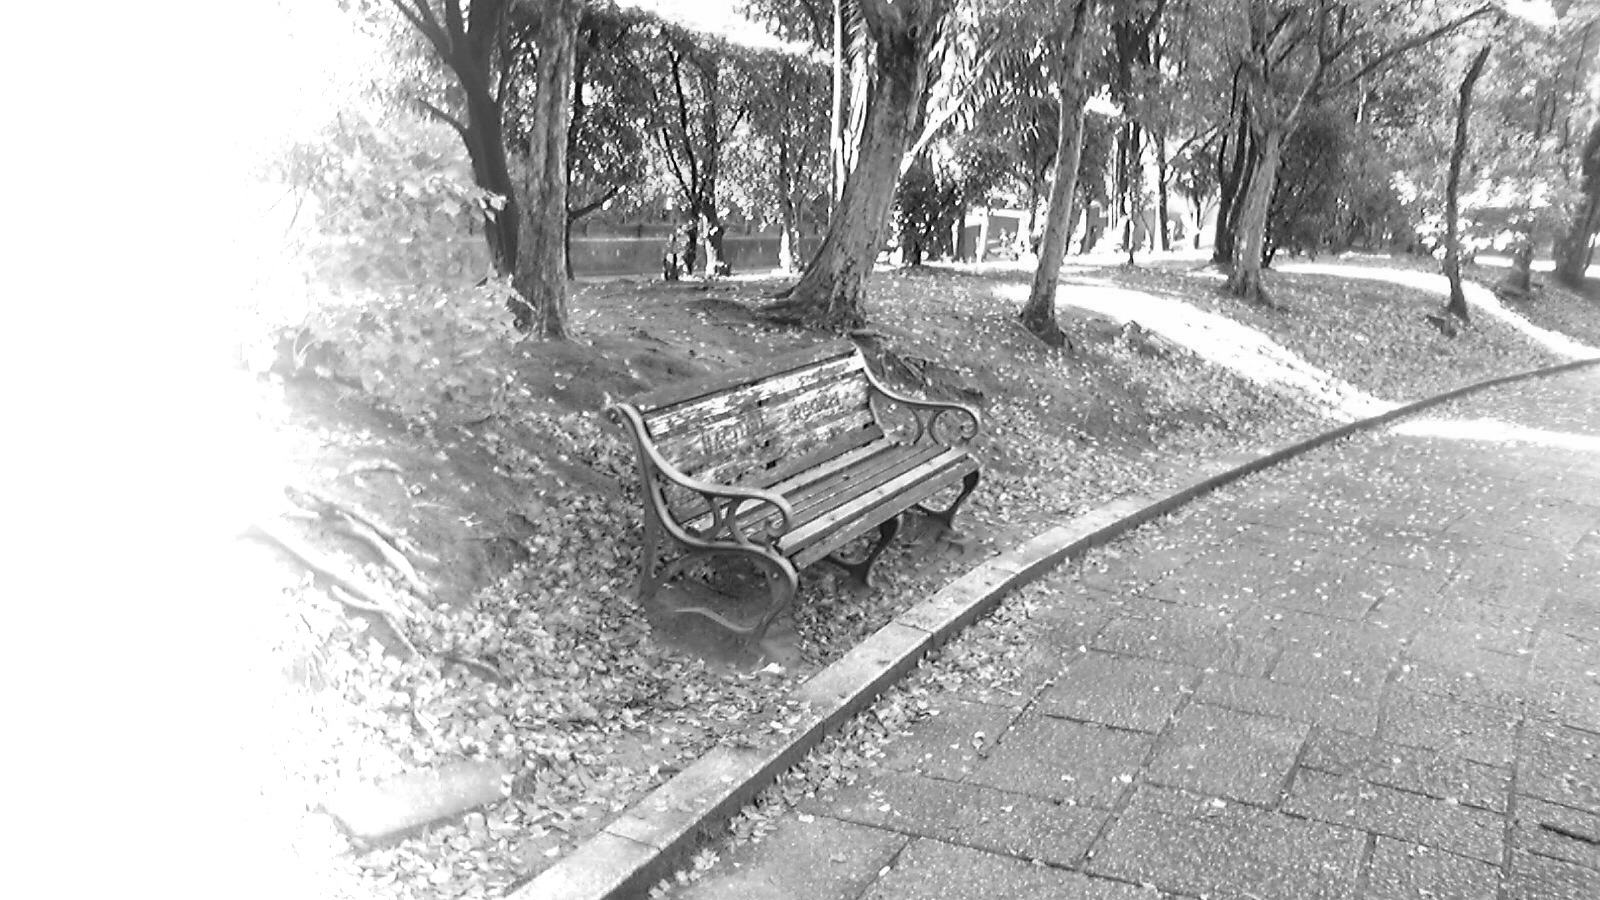
\includegraphics[width=0.58\textwidth,bb=0 0 1600 900]{img/park1.jpg}
\end{wrapfigure}

駅というのは普通、街の中心にあるものだ.
それは普通、駅を中心に街というのは発展するものだから.
だから駅より北方面、あるいは西側を私が知らないというのはいささか不思議である.
もちろん、いつもいつも、駅が街の中心というわけではない.
私が高校に通うのに使っていた岡本駅は、言ってしまえば六甲山の裾にあって、
駅より北には山しか無い.
というか駅が位置するその場所も、綺麗に舗装されてかなり気づきにくくはなっているものの、
山である.
まだ、山である、と言ったほうが正確か.
つまり、山というからには、山頂から地面は低い方低い方へと走っており、
その勢いは駅を通りすぎてもまだ止まらない.
駅から飛び出た人は、その安定したエネルギーを求めて、自然と足が南に向いてしまうという仕組みになっているのだ.
従って、この駅の場合、駅よりも南しか発展しない.
コンビニも雑貨屋もアイスクリーム屋も、南側にしか存在しない.

対して、この駅は、別になんということはない.
平地の上のぽんとあるだけである.
5分ほど東に歩いてみると大きな坂があって、実は高台にあったのだと気付くが、
しかし、
駅周辺だけを取り出してみれば、別段ただの平地である.
線路はほぼ東西に平行に走っており、
南側の駅口から入るとまず地下におり、そうして線路をくぐったのち、ホームに出る.
それよりも北側に何があるかなんてのは、
ホームから眺めれば分かることで、
なあんにもないのである.
この街に面白さを求めてはいけない.

一応、楽しいことといえば、
駅より10分ほど南に歩くと、割に大きな公園があって、
私は昼休みのほとんどをそこで過ごすのだが、
これはそんなに重要でないので省くことにする.

